\documentclass[12pt, a4paper]{article}
\usepackage[utf8]{inputenc}
\usepackage{amsmath}
\usepackage{amsfonts}
\usepackage{amsthm}
\usepackage{array}
\usepackage{graphicx}
\usepackage{parskip}
\usepackage[pdfencoding=auto]{hyperref}
\usepackage{fancyhdr}
\usepackage{lastpage}
\usepackage{tikz}
\usepackage{float}
\usepackage{listings}
\usepackage{color}
\usepackage{caption}
\usepackage{authblk}
\usepackage[acronym]{glossaries}
\usepackage[nottoc]{tocbibind}
\usepackage[cache=false]{minted}
\usemintedstyle{default}
\newminted{haskell}{frame=lines,framerule=2pt}
\newminted{R}{frame=lines,framerule=2pt}
\graphicspath{{./images/}}

\tikzstyle{bag} = [align=center]

\title{%
      Homework 6\\
      Network Dynamics Analysis\\
}
\author{Juan Pablo Royo Sales \& Francesc Roy Campderrós}
\affil{Universitat Politècnica de Catalunya}
\date\today

\pagestyle{fancy}
\fancyhf{}
\fancyhead[C]{}
\fancyhead[R]{UPC MIRI}
\fancyhead[L]{CSN - Homework 6}
\fancyfoot[L,C]{}
\fancyfoot[R]{Page \thepage{} of \pageref{LastPage}}
\setlength{\headheight}{15pt}
\renewcommand{\headrulewidth}{0.4pt}
\renewcommand{\footrulewidth}{0.4pt}

\newacronym{netdyn}{Network Dynamics}{Network Dynamics}
\newacronym{degdist}{Degree Distribution}{Degree Distribution}
\newacronym{growdeg}{Time Growth Degree}{Growth of Vertex Degree over time}
\newacronym{prefatt}{G Pref Attachment}{Growth + Preferential Attachment}
\newacronym{randatt}{G Random Attachment}{Growth + Random Attachment}
\newacronym{nprefatt}{NG Pref Attachment}{No Growth + Preferential Attachment}
\newacronym{baral}{Barabasi-Albert model}{Barabasi-Albert model}
\newacronym{indegree}{Incomming Degree}{Incomming Degree Language Set}
\newacronym{zeta}{Zeta}{Zeta Model}
\newacronym{aic}{Akaike}{Akaike Information Criterion}

\begin{document}

\maketitle

\tableofcontents

\section{Introduction}
In this homework we have analyzed \acrfull{netdyn} on different models proposed for this work.
The main goal of this work is to identify the best model which fit on both aspects of \acrshort{netdyn}, \acrfull{degdist} and \acrfull{growdeg}.
The following sections are going to show the results obtained and after that the discussion about the methodology used for the analysis and some conclusions at the end.

All the models that we have generated for the analysis of \acrfull{baral} over time have been done using \textbf{C++} Language and you can find the source code of this 
solution under \mintinline{shell}{code/main.cpp}.

The solution of this work is divided as follows:

\begin{itemize}
    \item \textbf{code}: Under this folder you are going to find \textit{C++} code for simulating and generating the different networks using the different strategies: \acrfull{prefatt}, \acrfull{randatt} and \acrfull{nprefatt}, as well as the \textit{R} scripts for generating plots and doing graph analysis.
    \item \textbf{code/data}: Data Generated for each strategy
    \item \textbf{report}: This report in Latex and PDF format.
\end{itemize}

\section{Results}
\subsection{Degree Distribution Analysis}\label{deg_dist_ana}
\subsubsection{Growth + Preferential Attachment}

\begin{table}[H]
    \centering
    \begin{tabular}{l r}
        Parameter & Value\\
        \hline              
        M & 200002\\
        N & 100002\\
        MAX & 1105\\
        M/N & 1.99\\
        N/M & 0.50\\
        MP & 37263.76\\
        C & 205119.83
    \end{tabular}
    \caption{Data Analysis over Growth + Pref Attachment}
    \label{table:grow_pref_att_1}
\end{table}

\begin{table}[H]
    \centering
    \begin{tabular}{l r}
        Distribution & Estimation\\
        \hline
        Displaced Poisson & 1.59\\
        Displaced Geometric & 0.50\\
        Zeta Gamma & 2.29\\ 
        Zeta Truncated & 103002\\
    \end{tabular}
    \caption{Estimation of Parameters: Growth + Pref Attachment}
    \label{table:grow_pref_att_2}
\end{table}

\begin{table}[H]
    \centering
    \begin{tabular}{l r}
        Distribution & AIC Value\\
        \hline
        Displaced Poisson & 253849.2\\
        Displaced Geometric & 33974.32\\
        Zeta Gamma 3 & 17100.8\\
        \textbf{Zeta Gamma} & \textbf{0}\\ 
        Zeta Truncated & 1.966677\\
    \end{tabular}
    \caption{AIC Selection: Growth + Pref Attachment}
    \label{table:grow_pref_att_3}
\end{table}

\begin{minipage}[t]{\linewidth}
    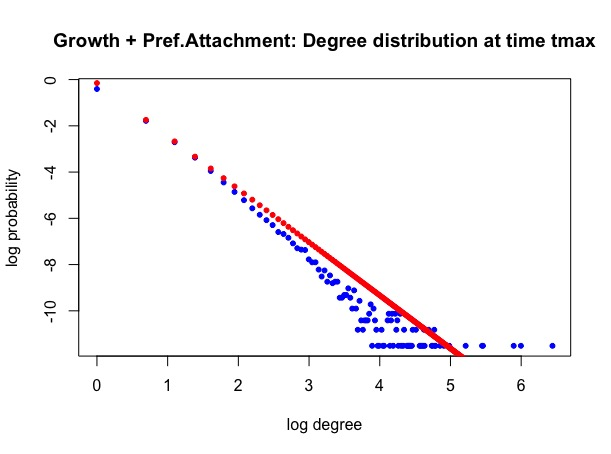
\includegraphics[width=\textwidth]{degree_tmax_grow_pref_att}
    \captionsetup{type=figure}
    \captionof{figure}{Degree $t_{max}$ Growth + Pref Att with Zeta $\Gamma = 3$}
    \label{fig:degree_tmax_grow_pref_att}
  \end{minipage}

\subsubsection{Growth + Random Attachment}

\begin{table}[H]
    \centering
    \begin{tabular}{l r}
        Parameter & Value\\
        \hline              
        M & 200002\\
        N & 100002\\
        MAX & 16\\
        M/N & 1.99\\
        N/M & 0.50\\
        MP & 50775.59\\
        C & 136242.14
    \end{tabular}
    \caption{Data Analysis over Growth + Random Attachment}
    \label{table:grow_ran_att_1}
\end{table}

\begin{table}[H]
    \centering
    \begin{tabular}{l r}
        Distribution & Estimation\\
        \hline
        Displaced Poisson & 1.59\\
        Displaced Geometric & 0.50\\
        Zeta Gamma & 2.07\\ 
        Zeta Truncated & 103002\\
    \end{tabular}
    \caption{Estimation of Parameters: Growth + Random Attachment}
    \label{table:grow_ran_att_2}
\end{table}

\begin{table}[H]
    \centering
    \begin{tabular}{l r}
        Distribution & AIC Value\\
        \hline
        Displaced Poisson & 82119.5\\
        \textbf{Displaced Geometric} & \textbf{0}\\
        Zeta Gamma 3 & 64197.51\\
        Zeta Gamma & 24921.01\\ 
        Zeta Truncated & 24922.54\\
    \end{tabular}
    \caption{AIC Selection: Growth + Random Attachment}
    \label{table:grow_ran_att_3}
\end{table}

\begin{minipage}[t]{\linewidth}
    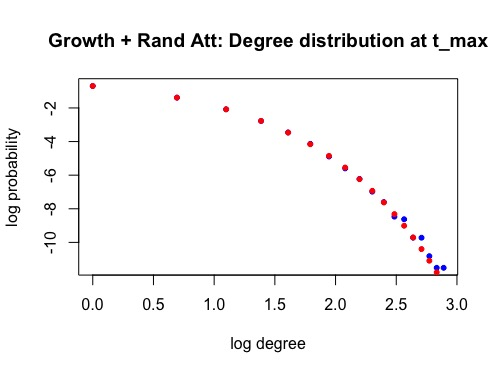
\includegraphics[width=\textwidth]{degree_tmax_grow_random_att}
    \captionsetup{type=figure}
    \captionof{figure}{Degree $t_{max}$ Growth + Pref Att with Displaced Geometric}
    \label{fig:degree_tmax_grow_pref_att}
  \end{minipage}

\subsection{Time Growth Degree Analysis}

\subsubsection{Growth + Preferential Attachment}

\begin{minipage}[t]{\linewidth}
    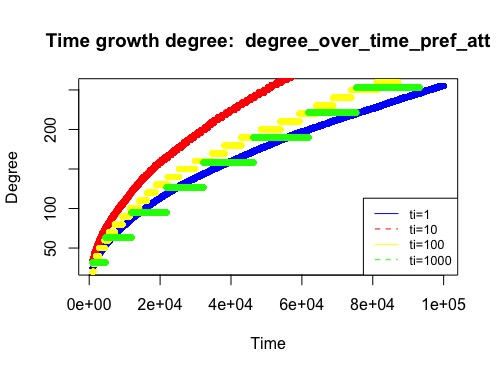
\includegraphics[width=\textwidth]{time_growth_degree_pref_att}
    \captionsetup{type=figure}
    \captionof{figure}{Time Growth Degree: Growth + Pref Att}
    \label{fig:time_growth_degree_pref_att}
  \end{minipage}

\begin{table}[H]
    \centering
    \begin{tabular}{l r}
        Model & AIC Value\\
        \hline
        Model 0  &  827909.63\\
        Model 1  &  98488.01\\
        Model 2  &  98043.99\\
        Model 3  &  696452.97\\
        Model 4  &  869213.48\\
        Model 0+  &  595689.50\\
        Model 1+  &  95483.67\\
        \textbf{Model 2+} & \textbf{82349.48}\\
        Model 3+  &  696467.54\\
        Model 4+  &  869216.84\\
    \end{tabular}
    \caption{AIC Selection: Growth + Preferential Attachment over Time Degree}
    \label{table:time_grow_ran_att_1}
\end{table}

\begin{minipage}[t]{\linewidth}
    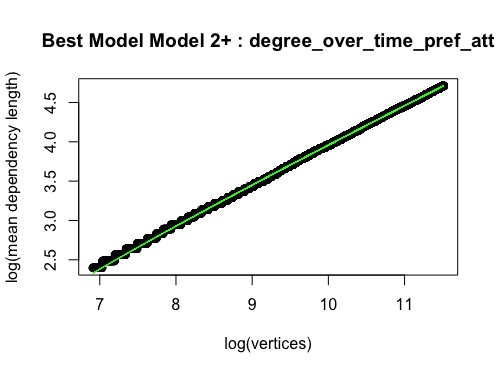
\includegraphics[width=\textwidth]{time_growth_degree_best_fit_pref_att}
    \captionsetup{type=figure}
    \captionof{figure}{Best Fit Time Growth Degree: Growth + Pref Att}
    \label{fig:time_growth_degree_best_fit_pref_att}
  \end{minipage}


\subsubsection{Growth + Random Attachment}

\begin{minipage}[t]{\linewidth}
    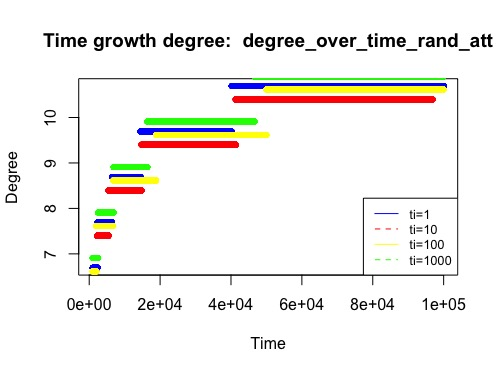
\includegraphics[width=\textwidth]{time_growth_degree_rand_att}
    \captionsetup{type=figure}
    \captionof{figure}{Time Growth Degree: Growth + Random Att}
    \label{fig:time_growth_degree_rand_att}
  \end{minipage}

\begin{table}[H]
    \centering
    \begin{tabular}{l r}
        Model & AIC Value\\
        \hline
        Model 0  &  529661.14\\
        Model 1  &  414515.14\\
        \textbf{Model 2}  &  \textbf{40943.69}\\
        Model 3  &  148894.78\\
        Model 4  &  60229.36\\
        Model 0+  &  140375.69\\
        Model 1+  &  89613.81\\
        Model 2+  & 45361.77\\
        Model 3+  &  148896.86\\
        Model 4+  &  60233.06\\
    \end{tabular}
    \caption{AIC Selection: Growth + Random Attachment over Time Degree}
    \label{table:time_grow_ran_att_1}
\end{table}


\begin{minipage}[t]{\linewidth}
    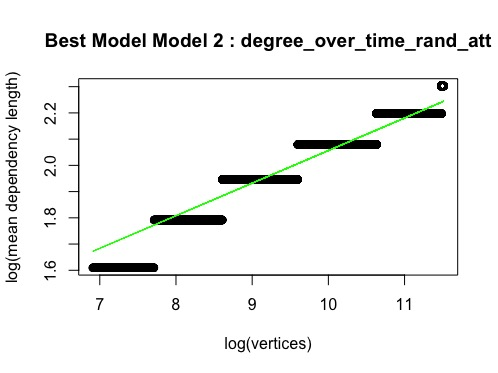
\includegraphics[width=\textwidth]{time_growth_degree_best_fit_rand_att}
    \captionsetup{type=figure}
    \captionof{figure}{Best Fit Time Growth Degree: Growth + Random Att}
    \label{fig:time_growth_degree_best_fit_rand_att}
  \end{minipage}

\section{Discussion and Methods}
\subsection{Methods}
As we have pointed out in the introduction we have use \textbf{C++} code for generating the different kinds of Growth in the \acrshort{baral}.
This can be found in the source code file \mintinline{shell}{code/main.cpp}. 

Regarding \textit{R} scripts we have the following scripts:

\begin{itemize}
    \item \mintinline{shell}{code/FromHomework2.R}: Which is the same script we have used on the Homework 2 for Fitting model analysis but we have change \acrshort{zeta} in order to fix $\Gamma = 3$
    \item \mintinline{shell}{code/Task1.R}: We have developed here the analysis and plotting of the first task about analysis of \acrshort{degdist}
    \item \mintinline{shell}{code/Task2.R}: We have developed here the analysis and plotting of the first task about analysis of \acrshort{growdeg}
\end{itemize}

\subsubsection{Parameters Selection}
Regarding the selection of parameters we have selected $m_0 = 1$, $n_0 = 2$, $t_{max} = 100.000$.
This selection is based on the fact that we have tried different kind of alternatives, but the only one which has given the best fit 
in~\ref{deg_dist_ana} is this set of parameters.

Other option that we have tested are:

\begin{itemize}
    \item $m_0 = 2$, $n_0 = 3$, $t_{max} = 100.000$
    \item $m_0 = 3$, $n_0 = 5$, $t_{max} = 100.000$
    \item $m_0 = 5$, $n_0 = 3$, $t_{max} = 100.000$
\end{itemize}

\subsection{Discussions}\label{sec:disc}
\subsubsection{Degree Distribution Analysis}
Regarding the \acrshort{degdist} analysis we can appreciate that for \acrshort{prefatt} we have checked that the best model that fits is the \acrshort{zeta} Distribution as
it is expected according to its \acrshort{aic} value and the plot obtained here~\ref{table:grow_pref_att_3} and here~\ref{fig:degree_tmax_grow_pref_att}.

\section{Conclusions}
As we have appreciated in the~\ref{sec:disc} .....

\end{document}

